\subsection{Validazione e collaudo}
\label{validazione_e_collaudo}
\textbf{Durata:} dal 2021\_05\_01 al 2021\_05\_19\\
Il periodo di validazione e collaudo inizia appena concluso il precedente e termina con la \glo{\textbf{RA}}.
Le precondizioni sono:
\begin{itemize}
    \item Le postcondizioni del periodo precedente sono state soddisfatte.
\end{itemize}
Le postcondizioni sono:
\begin{itemize}
    \item Aggiornamento e correzione documenti già prodotti;
    \item Esecuzione dei vari test;
    \item Completamento del prodotto in base a quanto discusso durante la \textbf{RQ};
    \item Consegna dei documenti richiesti in entrata alla \textbf{RA};
    \item Ultimata preparazione della presentazione da esporre in sede di revisione.
\end{itemize}
È composto da due incrementi e una nuova attività:
\begin{itemize}
    \item \textbf{Incremento e verifica dei documenti (dal 2021\_05\_01 al 2021\_05\_18)}: alcuni dei documenti già prodotti vengono migliorati e aggiornati ({\NdP}, {\PdP}, {\PdQ}, \textit{Manuale sviluppatore}, \textit{Manuale utente}); 
    \item \textbf{Incremento e verifica delle attività (dal 2021\_05\_01 al 2021\_05\_13)}: se necessario vengono migliorate le attività di \textbf{Technology Baseline} per quanto riguarda la progettazione ad alto livello, in particolare la \textbf{Product Baseline} riguardo all'aggiunta di design pattern o di diagrammi di classi o di attività; la parte di codifica comprende l'implementazione degli ultimi requisiti rimasti;
    \item \textbf{Validazione e collaudo (dal 2021\_05\_13 al 2021\_05\_19)}: realizzazione degli ultimi test, con successivi controlli finali per garantire un buon livello di qualità e correttezza.
\end{itemize}
\subsubsection{Incrementi del periodo}
\label{IncrementiValidazione}
\begin{table}[H]
	\begin{center}
		\begin{tabular}{ |C{3cm} C{6cm} C{7cm}| }
			\rowcolor{darkblue} 
			\textcolor{white}{\textbf{Incremento}} & \textcolor{white}{\textbf{Obiettivi}} & \textcolor{white}{\textbf{Requisiti}} \\ \hline
			I dal 2021\_05\_01 al 2021\_05\_13& Miglioramento della documentazione già prodotta, sviluppo ultimi requisiti & RFO68\_25 - RFO71\_25.3, RFO72\_26 \newline
			RFO73,
			RFO74,
			RFO75 \newline
			RFO76, RFO77, RFO78 \newline
			RFO101\_33, RFO102\_34 - RFO106\_34.4 \newline
			RF0107,  RFO108\_35, RFO109\_35.1 \newline 
			RFO110\_36, RFO111\_36.1, RFO112\_37 \newline
			RFO113\_38, RFO114 \newline RFO115\_39, RFO116\_39 \newline
			RFO117\_40,
			RFO118, RFO119\_41 \newline
			RFO120\_42, RFO121\_43 - RFO125\_43.2.2
			\\ \hline
			II dal 2021\_05\_13 al 2021\_05\_19 	& 
			Realizzazione ultimi test e controlli finali del prodotto e correzione dei documenti secondo la valutazione della \glo{RQ} & -\\ \hline
		\end{tabular}
		\caption{Tracciamento incrementi-obiettivi Validazione}
	\end{center}
\end{table}
\subsubsection{Ripianificazione attuata relativa al periodo} \label{RipianificazioneValidazione}
A seguito dei ritardi accumulati nei periodi precedenti si prevede di consegnare il prodotto verso metà maggio rispettando comunque il preventivo concordato precedentemente e il livello di qualità che il gruppo intende assicurare. Di seguito si riporta il nuovo diagramma di Gantt considerando la nuova data di consegna del prodotto.
\subsubsection{Diagramma di Gantt: Validazione e collaudo}\label{GanttValidazione}
\begin{figure}[ht]
    \centering
    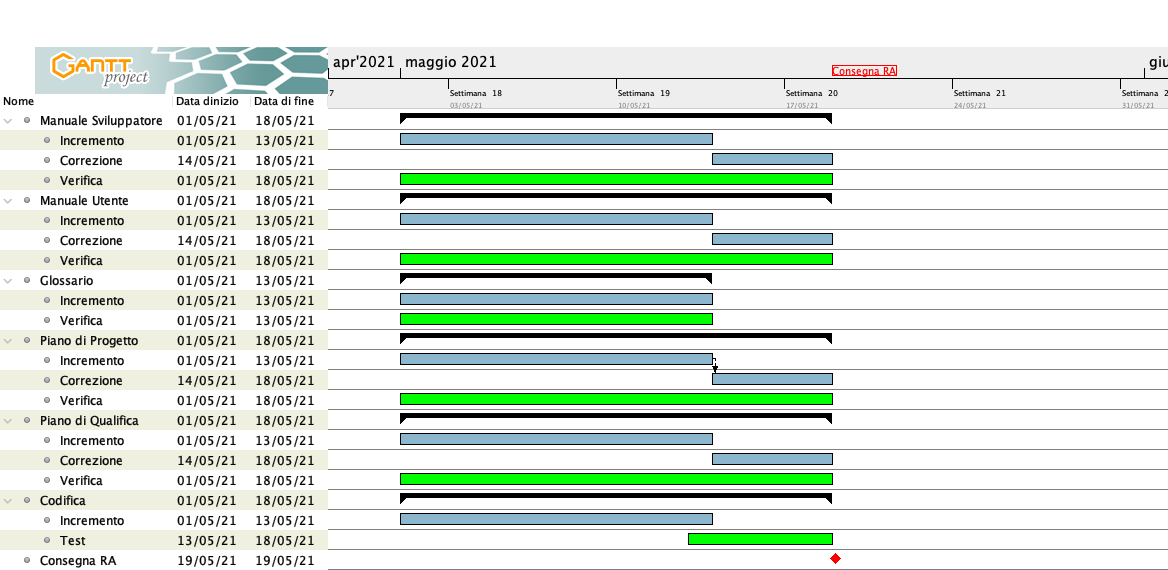
\includegraphics[width=\textwidth]{Immagini/GanttValidazione}
    \caption{Diagramma di Gantt dell'attività di validazione e collaudo}
\end{figure}